\documentclass[10pt]{article}

\usepackage[margin=1in]{geometry}
\usepackage{amsmath,amsthm,amssymb}
\usepackage{graphicx, wrapfig, subfig}

\usepackage{float}
\usepackage{multicol}
 \usepackage{booktabs}
 \usepackage{hyperref}
 \hypersetup{
 	colorlinks=true,
 	linkcolor=blue,
 	filecolor=magenta,      
 	urlcolor=cyan,
 }

\graphicspath{ {/Users/clay/Documents/research/TGE-SP21/assignments/images/} }

\begin{document}

% --------------------------------------------------------------
%                         Start here
% --------------------------------------------------------------

\title{Lecture 4 Worksheet}
\author{Geosc 597-003\\
Techniques of Geophysical Experimentation} 

\maketitle

\section*{Preparatory Reading}

\textcolor{red}{\textbf{\textit{Read about differential amplifiers before class:}}}
\begin{itemize}
	\item \url{https://www.electrical4u.com/differential-amplifier/}.
	\item INA105 Precision Unity Gain Differential Amplifier -- \textit{TGE-SP21/resources/INA105.pdf}
\end{itemize}


\section*{In-class Activity}
The goal of this activity is to learn about differential amplifier, feedback, and servo-control using the biaxial deformation apparatus in the Rock Mechanics Lab.\\

\begin{multicols}{2}
	\begin{figure}[H]
		\centering
		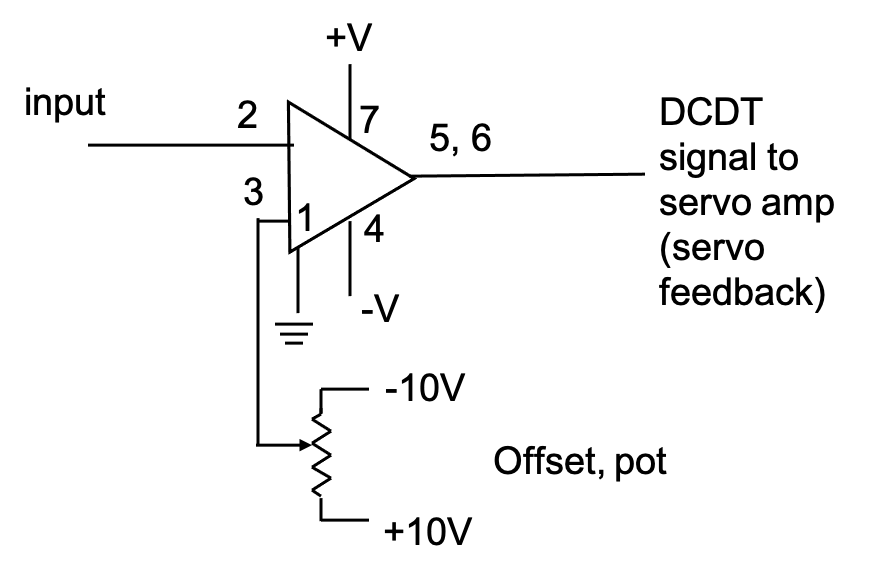
\includegraphics[width=\columnwidth]{dcdt_servo_feedback_diagram}
		\label{fig:dcdt_servo}
	\end{figure}
	
	\noindent\textbf{\textit{Displacement Control -- Vertical Ram:}}
	\begin{enumerate}
		\item Start with a balanced system, so that the servo error signal is zero. This means that the command and feedback are the same.
		\item \textbf{What is the output voltage of the DCDT?} \vspace{15pt}
		\item Now let’s look at what happens to the DCDT output when we offset the signal using just the offset pot.
		\item \textbf{After turning the pot 360° what is the output voltage of the DCDT?} \vspace{15pt}
		\item Is that what you expected?
		\item Now let’s lock the ram –or just turn off the hyd. power supply.  
		\item Turn the pot 360° -- what output voltage do you expect? \textbf{What is the measured output voltage of the DCDT?} \vspace{15pt}
	\end{enumerate}
\end{multicols}


\clearpage


\noindent\textbf{\textit{Servo Feedback -- Vertical Ram:}}
\begin{multicols}{2}
	
	\begin{figure}[H]
		\centering
		
\includegraphics[width=\columnwidth]{servo_feedback_diagram}
		\label{fig:servo_fdbk}
	\end{figure}
	
	\begin{enumerate}
		\item Where can the command originate?
		\item Where can the feedback originate?
		\item Let’s use \textit{Panel} for the command and \textit{Disp} for the feedback.
		\item Start with a balanced system, so that the servo error signal is zero.  This means that the command and feedback are the same.
		\item Increase the voltage to the command.
\textbf{What happens to the output voltage of the feedback (DCDT)?} \vspace{15pt}
		\item Now let’s send a continuously varying signal into the command: use \textit{Ext2} for the command and \textit{Disp} for the feedback.
		\item Start with a balanced system, so that the servo error signal is zero.  This means that the command and feedback are the same.
		\item Send in 10 digital counts per second.	W\textbf{hat happens to the output voltage of the feedback (DCDT)?} \vspace{15pt}
		\item Now look at what happens when we lock the system and change the command
		\item Use Ext2 for the command and Disp for the feedback.
		\item Start with a balanced system, so that the servo error signal is zero. This means that the command and feedback are the same.
		\item Lock the ram and then send in 1000 counts to the command.
		\item \textbf{Is it a good idea to unlock the ram right now? (yes/no)} \vspace{15pt}
		\item \textbf{What happens when you unlock?} \vspace{15pt}
		\item \textbf{What is the output voltage of the feedback (DCDT)? }\vspace{15pt}
	\end{enumerate}
\end{multicols}

\clearpage


\section*{Homework}
Analyze this circuit and determine the voltage at:

\begin{itemize}
	\item Pin 1 in switch position 1, 2, and 3.
	\item Pin 5 in switch position 1, 2, and 3.
\end{itemize}

\begin{figure}[ht]
	\centering
	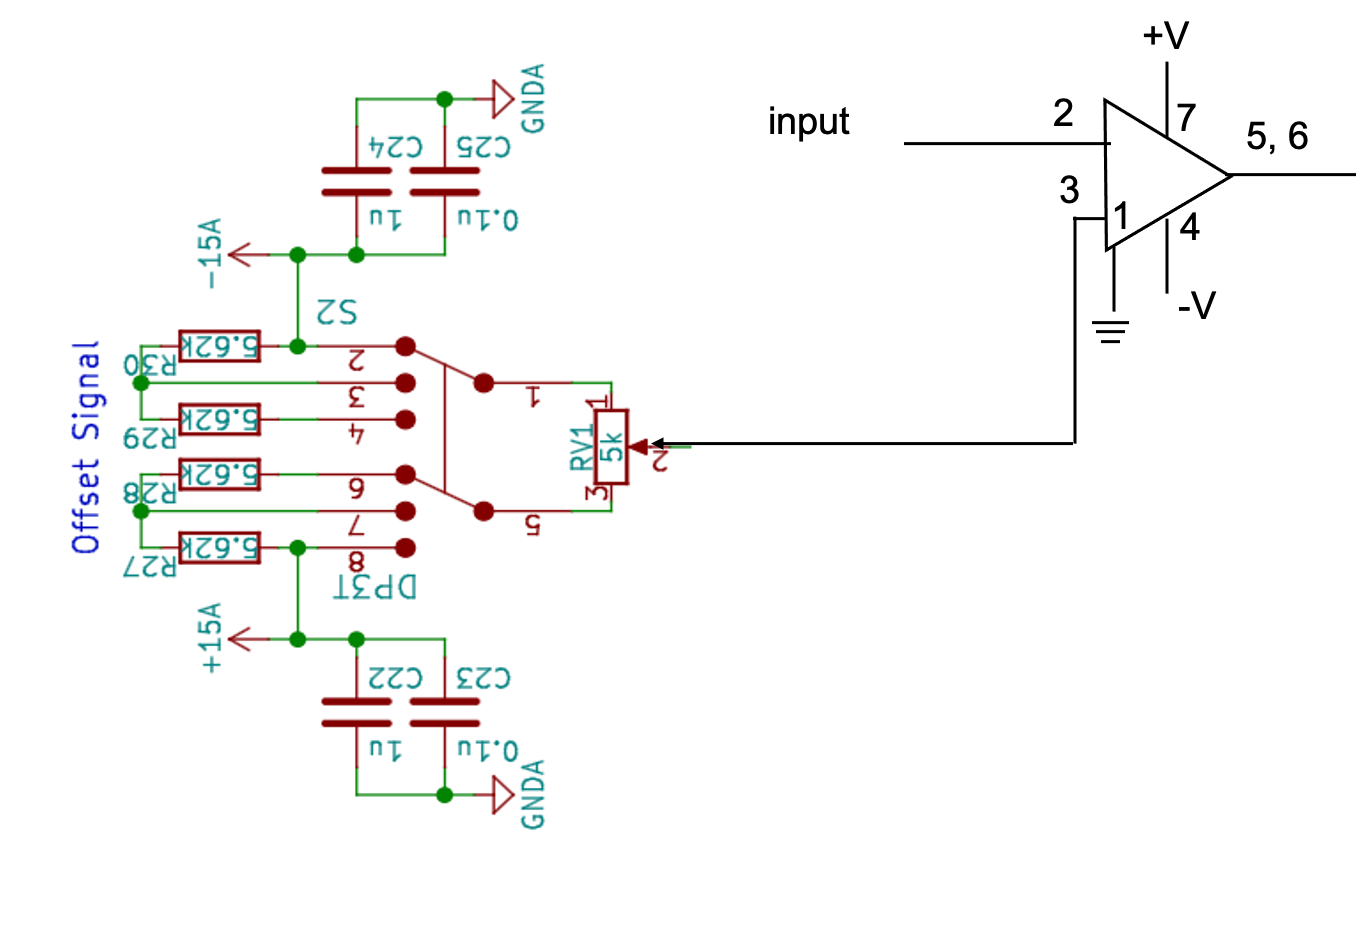
\includegraphics[width=0.8\columnwidth]{L4_hw_circuit}
\end{figure}


\end{document}